%%%%%%%%%%%%%%%%%%%%%%%%%%%%%%%%%%%%%%%%%%%%%%%%%%%%%%%%%%%%%%%%%%%%%%%%%%%%%%%%%%%%%%%%%%%%%%%%%%%
%%%%%%%%%%%%%%%%%%%%%%%%%%%%%%%%%%%%%%%%%%%%%%%%%%%%%%%%%%%%%%%%%%%%%%%%%%%%%%%%%%%%%%%%%%%%%%%%%%%
%%%%%%%%%%%%%%%%%%%%%%%%%%%%%%%%%%%%%%%%%%%%%%%%%%%%%%%%%%%%%%%%%%%%%%%%%%%%%%%%%%%%%%%%%%%%%%%%%%%

\chapter{Metodología y resultados}
\label{ch:metodologia}

El presente trabajo surge de una colaboración con el Laboratorio de Sueño, Emoción y Cognición, dependiente del Instituto de Ciencias de la Salud de la UAEH y a cargo de la Dra. Alejandra Rosales Lagarde.
%
La colaboración incluye acceso a los registros obtenidos en un estudio por Vázquez-Tagle en 2016 \cite{VazquezTagle16}. 
%
Dicho estudio se centró en la epidemiología de los trastornos del sueño en adultos mayores dentro del estado de Hidalgo, y consideró registros de PSG para evaluar parámetros relacionados al sueño MOR.
%
El presente trabajo tiene como objetivo particular analizar con mayor detalle dichos registros.

En este capítulo se describe primeramente la metodología seguida para obtener los registros de PSG.
%
Posteriormente se describe la metodología usada para analizar los registros de PSG, usando las herramientas descritas en el capítulo \ref{capitulo:espectro_evo}.

Los registros de PSG fueron segmentados en ventanas de 30 segundos, referidas como \textbf{épocas}.
%
El análisis de los registros de PSG se llevó a cabo a tres niveles:
\begin{itemize}
\item Dentro de cada época.
\item Entre las diferentes épocas en un registro.
\item Entre los diferentes participantes.
\end{itemize}

El análisis a nivel de época contempla su clasificación según etapa de sueño (limitada a MOR y NMOR), y su clasificación como estacionarias (usando la prueba de PSR).
%
El uso de épocas como unidades de estudio se justifica por la gran heterogeneidad del sueño nocturno; paralelamente, destaca el supuesto fisiológico de que las etapas de sueño son \textit{comunes} entre los humanos.
%
En suma, los registros de PSG para un sólo individuo pueden interpretarse como una población de épocas.
%; en una misma etapa de sueño, las épocas de dos individuos cualesquiera son comparables.

El análisis a nivel de registro surge de considerar la heterogeneidad del sueño pero usando al registro entero como unidad de estudio.
%
%Aún antes de comparar los registros de diferentes sujetos, se hallaron algunos patrones interesantes de actividad en los registros. 
%, que revelan información sobre la estructura de estos registros. 
%
El tomar las épocas junto con su estructura temporal reveló algunos patrones interesantes de actividad.

Para el análisis entre participantes (divididos en grupos), varias de las características descritas fueron \textit{colapsadas} para constituir características \textit{simples}. 
%
%Como ejemplo, se calculó el porcentaje de épocas MOR que también fueron clasificadas como estacionarias; dicha 
%
Debido a las características de la muestra (ver más adelante), los resultados obtenidos no pueden extrapolarse a la población en general.
%
Los resultados obtenidos, entonces, se presentan como \textit{indicios}.

%%%%%%%%%%%%%%%%%%%%%%%%%%%%%%%%%%%%%%%%%%%%%%%%%%%%%%%%%%%%%%%%%%%%%%%%%%%%%%%%%%%%%%%%%%%%%%%%%%%

\section{Características de los participantes}

Los participantes fueron elegidos usando un muestreo \textit{no probabilístico por conveniencia} bajo los siguientes criterios de inclusión:
\begin{itemize}
\item Edad entre 60 y 85 años
\item Diestros (mano derecha dominante)
\item Sin ansiedad, depresión ni síndromes focales
\item No usar medicamentos o sustancias para dormir
\item Firma de consentimiento informado
\item Voluntario para el registro de PSG
\end{itemize}

Un total de 16 adultos mayores cumplieron los criterios de inclusión. 
%
Con el fin de detectar el DCL en estos pacientes, éstos fueron sometidos a una batería de pruebas neuropsicológicas para determinar su estado cognoscitivo general (Neuropsi, MMSE), detectar cambios en su vida cotidiana (KATZ) y descartar cuadros depresivos (SAST, GDS); para más detalles ver capítulo anterior, sección \ref{seccion:pruebas}.
%
%En las tablas ??--?? se resumen las puntuaciones que pueden obtenerse en las pruebas mencionadas, así como de qué son indicativos; 
%
En la tabla \ref{puntajes} se reportan los puntajes obtenidos por los participantes en dichas pruebas.
%
Se determinó que, objetivamente, 12 de los voluntarios no padecen depresión o ansiedad, ni presentan afectaciones significativas en la vida diaria.
%
Debido a problemas técnicos diversos, sólo 9 participantes fueron considerados; se reportan únicamente los datos relativos a esos participantes.

En base al diagnóstico de Posible Deterioro Cognitivo Leve, los 9 participantes fueron divididos en dos grupos: PDCL y CTRL. 
%
Es importante mencionar que, bajo las condiciones muestrales, el grupo CTRL no puede fungir satisfactoriamente como grupo control; una descripción más adecuada sería \textit{grupo sin PDCL}.

%Para esta clasificación se dio mayor atención al puntaje de Neuropsi, estandarizado según edad y 
%escolaridad (cuadro \ref{puntajes}). 
%
%Cabe mencionar que intencionalmente se dio menor importancia a los puntajes de la prueba MMSE en cuanto al diagnóstico del PDCL; ésto porque se ha reportado que, en la población mexicana, esa prueba tiene baja sensibilidad para el diagnóstico de DCL en general, y baja especificidad para individuos con escolaridad muy baja o muy alta \cite{Ostrosky00}.
%%
%Para fines del comentario anterior, se entiende por \textit{sensibilidad} a la probabilidad de obtener verdaderos positivos, y por \textit{especificidad} a la probabilidad de obtener verdaderos negativos.

%\begin{table}
%\caption{Datos generales de los participantes}
%\centering
%\bordes{1.1}
%{\small
%\begin{tabular}{llcrrrrrrr}
%\toprule
% \phantom{.}&
% & {Sexo} & {Edad} & {Escol.} & {Neuropsi} & {MMSE} & {SAST} & {KATZ} & {GDS} \\
%\midrule
%\multicolumn{6}{l}{\textbf{Grupo CTL}}\\
%&VCR    & F    & 59\pz & 12\pz & 107\pz & 29\pz & 21\pz & 0\pz & 3\pz \\
%&MJH    & F    & 72\pz & 9\pz  & 113\pz & 30\pz & 18\pz & 0\pz & 0\pz \\
%&JAE    & F    & 78\pz & 5\pz  & 102\pz & 28\pz & 19\pz & 0\pz & 5\pz \\
%&GHA    & M    & 65\pz & 9\pz  & 107.5  & 30\pz & 23\pz & 0\pz & 7\pz \\
%&MFGR   & F    & 67\pz & 11\pz & 115\pz & 30\pz & 18\pz & 0\pz &      \\
%\rowcolor{gris}
%&\multicolumn{1}{c}{$\widehat{\mu}$} & 
%               & 68.2  & 9.2   & 108.9  & 29.4  & 19.8  & 0.0  & 3.0  \\
%\rowcolor{gris}
%&\multicolumn{1}{c}{$\widehat{\sigma}$} & 
%               & 7.2   & 2.7   & 5.2    & 0.9   & 2.2   & 0.0  & 3.0  \\
%\midrulec
%%\hline
%\multicolumn{6}{l}{\textbf{Grupo PDC}}\\
%&CLO    & F    & 68\pz & 5\pz  & 81\pz & 28\pz & 22\pz & 1\pz & 6\pz \\
%&RLO    & F    & 63\pz & 9\pz  & 90\pz & 29\pz & 20\pz & 0\pz & 3\pz \\
%&RRU    & M    & 69\pz & 9\pz  & 85\pz & 27\pz & 10\pz & 0\pz & 3\pz \\
%&JGZ    & M    & 65\pz & 11\pz & 87\pz & 25\pz & 20\pz & 0\pz & 1\pz \\
%&AEFP   & M    & 73\pz &  8\pz & 96\pz & 29\pz &   \pz & 0\pz & 2\pz \\
%\rowcolor{gris}
%&\multicolumn{1}{c}{$\widehat{\mu}$} & 
%              & 67.6   & 8.4   & 87.8  & 27.4  & 18.0  & 0.2  & 3.0  \\
%\rowcolor{gris}
%&\multicolumn{1}{c}{$\widehat{\sigma}$} & 
%              & 3.4    & 2.2   & 5.6   & 1.8   & 5.4   & 0.4  & 1.9  \\
%\bottomrulec
%\end{tabular} 
%}
%\label{tab_sujetos}
%\end{table}

\begin{table}
\caption{Datos generales de los participantes}
\centering
\bordes{1.1}
{\small
\begin{tabular}{llcrrrrrrr}
\toprule
 \phantom{mmm}&
 & {Sexo} & {Edad} & {Escol.} & {Neuropsi} & {MMSE} & {SAST} & {KATZ} & {GDS} \\
\midrule
\multicolumn{2}{l}{\textbf{Grupo CTRL}}\\
&MJH    & F    & 72\pz & 9\pz  & 113\pz & 30\pz & 18\pz & 0\pz & 0\pz  \\
&JAE    & F    & 78\pz & 5\pz  & 102\pz & 28\pz & 19\pz & 0\pz & 5\pz  \\
&MGG    & F    & 61\pz & 9\pz  & 114\pz & 28\pz & 29\pz & 1\pz & 14\pz \\
&EMT    & F    & 50\pz & 22\pz & 117\pz & 30\pz & 15\pz & 0\pz & 4\pz  \\
\rowcolor{gris}
&\multicolumn{1}{c}{$\widehat{\mu}$} & 
               & 65.3  & 11.3  & 111.5  & 29.0  & 20.3  & 0.3  & 5.8  \\
\rowcolor{gris}
&\multicolumn{1}{c}{$\widehat{\sigma}$} & 
               & 12.4  & 7.4   & 6.6    & 1.2   & 6.1   & 0.5  & 5.9  \\
\midrulec
%\hline
\multicolumn{2}{l}{\textbf{Grupo PDCL}}\\
& CLO   & F    & 68\pz &  5\pz &  81\pz & 28\pz & 22\pz & 1\pz &  6\pz \\
& RLO   & F    & 63\pz &  9\pz &  90\pz & 29\pz & 20\pz & 0\pz &  3\pz \\
& JGZ   & M    & 65\pz & 11\pz &  87\pz & 25\pz & 20\pz & 0\pz &  1\pz \\
& AEFP  & M    & 73\pz &  8\pz &  96\pz & 29\pz &   \pz & 0\pz &  2\pz \\
& PCM   & M    & 71\pz &  9\pz & 111\pz & 28\pz & 20\pz & 0\pz & 10\pz \\
\rowcolor{gris}
&\multicolumn{1}{c}{$\widehat{\mu}$} & 
              &  68.0  & 8.4   & 93.0   & 27.8  & 20.5  & 0.2  & 4.4  \\
\rowcolor{gris}
&\multicolumn{1}{c}{$\widehat{\sigma}$} & 
              & 4.1    & 2.2   & 11.4   & 1.6   & 1.0   & 0.4  & 3.6 \\
\bottomrulec
\end{tabular} 
}
\label{tab_sujetos}
\end{table}

%%%%%%%%%%%%%%%%%%%%%%%%%%%%%%%%%%%%%%%%%%%%%%%%%%%%%%%%%%%%%%%%%%%%%%%%%%%%%%%%%%%%%%%%%%%%%%%%%%%
%%%%%%%%%%%%%%%%%%%%%%%%%%%%%%%%%%%%%%%%%%%%%%%%%%%%%%%%%%%%%%%%%%%%%%%%%%%%%%%%%%%%%%%%%%%%%%%%%%%

\subsection{Registro del polisomnograma}

Para efectuar el registro de la PSG, los participantes acudieron a las instalaciones del Laboratorio de Sueño, Emoción y Cognición. 
%
Los participantes recibieron instrucciones de realizar una rutina normal de actividades durante la semana que precedió al estudio, y se les recomendó no ingerir bebidas alcohólicas o energizantes (como café o refresco) durante las 24 horas previas al experimento, y que no durmieran siesta ese día.
%
Bajo estas condiciones experimentales se garantiza que los registros son representativos del sueño nocturno de cada participante.

El registro per se fue efectuado usando un polisomnógrafo Medicid 5 (Neuronic Mexicana). El protocolo de la PSG incluye los siguientes electrodos\footnote{Para más detalles ver el capítulo anterior, particularmente la sección \ref{capitulo:psg}}:
\begin{itemize}
\item 19 electrodos de EEG colocadas según el Sistema Internacional 10--20.
\item 2 electrodos de EOG para movimientos oculares.
\item 2 electrodos de EMG para tono muscular en los músculos submentonianos.
\end{itemize}

Los electrodos para EEG fueron conectados en paralelo usando como referencia común los lóbulos de las orejas; se mantuvo por debajo de \SI{50}{\micro\ohm}.
%
Las señales fueron amplificadas analógicamente usando amplificadores de alta ganancia en cadena, 
y adicionalmente fueron \textit{pasado} filtros analógicos pasa bandas: 0.1--100 Hz 
para EEG, 3--20 Hz para EOG. 
%Debido a dificultades técnicas el registro se efectuó a razón de 512 puntos por segundo (Hz) para 
%algunos participantes, mientras que se usó 200 Hz para otros; en ambos casos se cumple la 
%recomendación de la AASM de al menos 128 Hz.
%
Los registros fueron digitalizados con una frecuencia de muestreo de 512 puntos por segundos (Hz), y posteriormente almacenados en formato de texto bajo la codificación ASCII.

Como se mencionó anteriormente, los registros fueron segmentados en segmentos de 30 segundos, referidas como 
\textbf{épocas}.
%, para su estudio posterior \textit{fuera de línea}. 
Cada una de las épocas fue clasificada como MOR o NMOR; la clasificación fue llevada a cabo por dos expertos de ICSA, y bajo los estándares de la AASM.

Por simplicidad técnica, los registros fueron truncados para poder considerar épocas completas; algunos datos al final de cada registro fueron omitidos, aunque representan una cantidad negligible de tiempo.
%
Cabe mencionar que cada época de 30 segundos, a una frecuencia de 512 Hz, representa un total de 15,360 puntos.

En la tabla \ref{tab:psg} se describe la duración de los registros, así como la cantidad de tiempo del registro clasificado como sueño MOR.
%
La cantidad de tiempo en vigilia registrado es negligible ($<5$ minutos por cada participante), de modo que ésta no es reportada; con una pérdida mínima de generalidad, se puede afirmar que los registros fuera del sueño MOR corresponden a sueño NMOR.

\begin{table}
\centering
\caption{Datos generales sobre los registros de PSG}
\bordes{1.2}
\begin{tabular}{llllcllr}
\toprule
    \phantom{mmm}&
    & \multicolumn{2}{l}{Total} & \phantom{l}   & \multicolumn{3}{l}{MOR*}\\
    \cmidrule{3-4}  \cmidrule{6-8}
    &          &Épocas  &  Tiempo   &&Épocas  &  Tiempo   &  \% \\
\midrule
\multicolumn{2}{l}{\textbf{Grupo CTL}}\\
&MJH &    1032   &      8:36:00  &&    127   &   1:03:30 &12.31 \\
&JAE &\ppu 904   &      7:32:00  &&    171   &   1:25:30 &18.92 \\
&MGG &    1024   &      8:32:00  &&    166   &   1:23:00 &16.21 \\
&EMT &\ppu 552   &      4:36:00  &&\ppu 47   &   0:23:00 & 8.51 \\
 
\rowcolor{gris}
&\multicolumn{1}{c}{$\widehat{\mu}$}  
     &\ppu 878.0 &      7:19:00 &&    128.0 &   1:03:53&13.99 \\
\rowcolor{gris}
&\multicolumn{1}{c}{$\widehat{\sigma}$} 
     &\ppu 225.1 &      1:52:32 &&\ppu 57.3  &   0:28:39&4.55 \\ 
\midrulec

\multicolumn{2}{l}{\textbf{Grupo PDC}}\\
&CLO  &\ppu 944   &\ppu 7:52:00 &&    132   &   1:06:00 & 13.98 \\
&RLO  &\ppu 840   &\ppu 7:00:00 &&\ppu 99   &   0:49:30 & 11.79 \\
&JGZ  &    1200   &    10:00:00 &&\ppu 34   &   0:17:00 &  2.83 \\
&AEFP &\ppu 952   &\ppu 7:56:00 &&\ppu 41   &   0:20:00 &  4.31 \\
&PCM  &\ppu 752   &\ppu 6:16:00 &&\ppu 59   &   0:29:30 &  7.85 \\
 
\rowcolor{gris}
&\multicolumn{1}{c}{$\widehat{\mu}$}  
      &\ppu 937.6 &\ppu 7:48:48 &&\ppu 73.0 &   0:36:30 & 8.15 \\
\rowcolor{gris}
&\multicolumn{1}{c}{$\widehat{\sigma}$} 
      &\ppu 168.1 &\ppu 1:24:04 &&\ppu 41.5 &   0:20:46 & 4.75 \\
\bottomrulec
\end{tabular}\\
*El sueño MOR aparece fragmentado, se reporta la suma de tales tiempos
\label{tab:psg}
\end{table}

%%%%%%%%%%%%%%%%%%%%%%%%%%%%%%%%%%%%%%%%%%%%%%%%%%%%%%%%%%%%%%%%%%%%%%%%%%%%%%%%%%%%%%%%%%%%%%%%%%%
%%%%%%%%%%%%%%%%%%%%%%%%%%%%%%%%%%%%%%%%%%%%%%%%%%%%%%%%%%%%%%%%%%%%%%%%%%%%%%%%%%%%%%%%%%%%%%%%%%%

\section{Características muestrales}

Previo a los análisis de los registros de PSG, se corroboró si los dos grupos de participantes efectivamente se \textit{comportan} como grupos estadísticamente diferentes.
%
Con dicho objetivo, se aplicaron pruebas $U$ de Wilcoxon-Mann-Whithney (WMW) entre los dos grupos, para todas las variables consideradas. 
%
De lo anterior se exceptúa al puntaje de la prueba KATZ, ya que es un parámetro cualitativo. 
%
Se concluye que las mediciones son parecidas en ambos grupos para todas las variables observadas, excepto para el puntaje en la prueba Neuropsi; ello era de esperarse ya que el puntaje en Neuropsi fue usado para designar a los participantes en los grupos.
%
Los resultados de estas pruebas se reportan en la tabla \ref{tab:var_wilcox}.

\begin{table}
\centering
\caption{Variables independientes entre grupos}
\begin{tabular}{lrlcrlcccr}
\toprule
 & \multicolumn{2}{l}{Grupo CTRL} & \phantom{.} & \multicolumn{2}{l}{Grupo PDCL} 
 & \phantom{.} & \multicolumn{2}{l}{Prueba de WMW}
 \\
\cmidrule{2-3} \cmidrule{5-6} \cmidrule{8-9}
& Media & (DE) & & Media & (DE) & & $p$ & $W$ \\
\midrule
Edad          & 65.3     & 12.4     &      & 68.0     & 4.1      &        & 0.905 & 9.0  \\
Escolaridad   & 11.3     & 7.4      &      & 8.4      & 2.2      &        & 0.797 & 11.5 \\
Neuropsi      & 111.5    & 6.6      &      & 93.0     & 11.4     &        &\bf 0.032 & 19.0 \\
MMSE          & 29.0     & 1.2      &      & 27.8     & 1.6      &        & 0.366 & 14.0 \\
SATS          & 20.3     & 6.1      &      & 20.5     & 1.0      &        & 0.301 & 4.0  \\
GDS           & 5.8      & 5.9      &      & 4.4      & 3.6      &        & 0.905 & 11.0 \\
Sueño {[}s{]} & 7:19:00  & 1:52:32  &      & 7:48:48  & 1:24:04  &        & 1.000 & 10.0 \\
MOR {[}s{]}   & 1:03:52  & 0:28:39  &      & 0:36:30  & 0:20:46  &        & 0.190 & 16.0 \\
MOR {[}\%{]}  & 14.0\%   & 4.5\%    &      & 8.2\%    & 4.8\%    &        & 0.111 & 17.0 \\
\bottomrule 
\multicolumn{8}{l}{DE=Desviación Estándar, WMW=Wilcoxon--Mann--Whitney}
\end{tabular} 
\label{tab:var_wilcox}
\end{table}

%Así mismo, se verificó si las variables medias (edad, escolaridad, puntajes en las pruebas) estaban correlacionadas entre sí.

%Previo al análisis de la estacionariedad, se corroboró la hipótesis de que las variables 
%independientes son estadísticamente iguales entre los grupos CTL y PDC. Las comparaciones
%usando la prueba $t$ de Welch (cuadro \ref{var_ind}) indican que efectivamente la hipótesis se cumple salvo
%para los puntajes de Neuropsi.

Se verificó si hay correlaciones entre las variables consideradas, lo cual podría afectar la interpretación de los resultados posteriores.
%
Para ello se aplicó la prueba de correlación de Spearman a cada par de variables; para la prueba de Spearman estima de la correlación entre variables, y se prueba la hipótesis de que la correlación es diferente de cero.
%
Estos resultados se reportan en el cuadro \ref{tab:correlacion}.

\begin{table}
\centering
\caption{Prueba de correlación de Spearman (estimación y p-valor)}
\begin{tabular}{ccccccccc}
\toprule
             & \rotatebox{90}{Escolaridad} & \rotatebox{90}{Neuropsi} & \rotatebox{90}{MMSE} & \rotatebox{90}{SAST} & \rotatebox{90}{GDS} & \rotatebox{90}{Sueño [s]} & \rotatebox{90}{MOR [s]} & \rotatebox{90}{MOR [\%]} \\
\midrule
Edad     & -0.699 & -0.267 & -0.079 & -0.171 & -0.233 & 0.200  & 0.183  & 0.100   \\
         & (0.04) & (0.49) & (0.84) & (0.69) & (0.55) & (0.61) & (0.64) & (0.81)  \\
\rowcolor{gris}
Escol.   &        & 0.437  & 0.194  & -0.366 & -0.254 & -0.044 & -0.586 & -0.525  \\
\rowcolor{gris}
         &        & (0.24) & (0.62) & (0.37) & (0.51) & (0.91) & (0.10) & (0.15)  \\

Neuropsi &        &        & 0.501  & -0.415 & 0.200  & -0.267 & 0.150  & 0.200   \\
         &        &        & (0.17) & (0.31) & (0.61) & (0.49) & (0.71) & (0.61)  \\

\rowcolor{gris}
MMSE     &        &        &        & -0.628 & -0.378 & -0.316 & -0.070 & 0.018   \\
\rowcolor{gris}
         &        &        &        & (0.09) & (0.32) & (0.41) & (0.86) & (0.96)  \\

SATS     &        &        &        &        & 0.610  & 0.317  & 0.293  & 0.195   \\
         &        &        &        &        & (0.11) & (0.44) & (0.48) & (0.64)  \\

\rowcolor{gris}
GDS      &        &        &        &        &        & -0.433 & 0.517  & 0.467   \\
\rowcolor{gris}
         &        &        &        &        &        & (0.25) & (0.16) & (0.21)  \\

Sueño [s]&        &        &        &        &        &        & -0.050 & -0.067  \\
         &        &        &        &        &        &        & (0.91) & (0.88)  \\

\rowcolor{gris}
MOR [s]  &        &        &        &        &        &        &        & 0.983   \\
\rowcolor{gris}
         &        &        &        &        &        &        &        & (0.00)  \\
%\bottomrule
\bottomrulec
%\multicolumn{7}{l}{Niveles de significancia: *$<$.05 , **$<$.01 , ***$<$.005 , ****$<$.001}
\end{tabular}
\label{tab:correlacion}
\end{table}

Sólo se encontraron correlaciones significativas entre dos pares de variables: edad y escolaridad, y tiempo en MOR \textit{medido} en segundos y en porcentaje.

La primera relación, no muy fuerte, puede explicarse como un \textit{efecto generacional}: la educación superior ha aumentado su cobertura durante las últimas décadas, y entonces los grupos poblacionales más jóvenes tienen en promedio más años de escolaridad. 
%
%En base a estudios horizontales de larga escala, algunos autores han sugerido que un bajo nivel de escolaridad es un factor de riesgo para padecer deterioro cognitivo \cite{Mejia_Arango2007}.
%%
%En vista que para el grupo de participantes no se pudo relacionar el nivel de escolaridad con el desempeño en las pruebas neuropsicológicas, dicha hipótesis no será explorada.
%
Una segunda hipótesis para esta correlación es la contribución del participante EMT, quien tiene una edad menor y un nivel de educación mayor al resto de los participantes.
%
Para contrastar la segunda hipótesis se calculó nuevamente la prueba de Spearman pero retirando los datos de EMT: se halló una correlación estimada de 0.179 con un p-valor asociado de 0.672, que no permite rechazar el que la correlación sea diferente de cero.

Se descarta entonces la hipótesis del efecto generacional, cuando menos para el grupo de participantes considerados, y se acepta que la correlación es debida a valores atípicos. Se concluye que, usando los datos recabados, no se pueden obtener información relevante sobre el efecto del nivel de educación ni la edad sobre el PDCL, ni con los marcadores del PSG que se describirán más adelante.

Intuitivamente era de esperarse la correlación entre el tiempo en MOR y el porcentaje de sueño que es MOR.
%
Sin embargo, la hipótesis de que el sueño tenga una \textit{estructura característica} --y por tanto, que las etapas de sueño aparezcan en proporciones similares en varios individuos--- es ajena a los supuestos estadísticos.
%
Con base a este resultado, en adelante se usará el porcentaje de MOR como \textit{sustituto} del tiempo real de MOR porque (1) dichas variables están fuertemente correlacionadas, y (2) porque el porcentaje permite comparar intuitivamente a características de registros con duraciones muy diferentes.

%Usando la prueba de correlación de Spearman (cuadro \ref{cor_ind}) se encontró sólo hay 
%correlaciones monotónicas entre los siguientes pares de variables:
%\begin{itemize}
%\item Edad y Escolaridad
%\item Puntaje en Neuropsi y Puntaje en Mini Mental-State Examination (MMSE)
%\item Tiempo de MOR (en segundos) y Tiempo en MOR (porcentaje)
%\end{itemize}
%
%La primera relación, no muy fuerte, puede explicarse como un \textit{efecto generacional}: la educación 
%superior ha aumentado su cobertura durante las últimas décadas, y entonces los grupos poblacionales 
%más jóvenes tienen en promedio más años de escolaridad. 
%%
%Algunos autores han sugerido que un bajo nivel de escolaridad es un factor de riesgo para padecer
%deterioro cognitivo, en base a estudios horizontales de larga escala \cite{Mejia_Arango2007}.
%%
%En el presente trabajo se ignora este dato, en vista de que no se pudieron relacionar el nivel de 
%escolaridad de los participantes con su desempeño en pruebas neuropsicológicas.
%
%La relación entre los puntajes en Neuropsi y en MMSE era de esperarse, ya que ambas pruebas miden
%parámetros similares y tienen contenidos independientes. Cabe mencionar el curioso fenómeno en que (1) 
%los puntajes de MMSE
%tienen estadísticamente las mismas medias grupales, (2) los puntajes de MMSE están 
%fuertemente correlacionados con los puntajes de Neuropsi, y (3) los puntajes de Neuropsi
%tienen estadísticamente medias grupales diferentes. Se confirma que la prueba MMSE
%tiene menor sensibilidad que la prueba Neuropsi para detectar deterioro cognitivo.
%
%Era por demás obvia la relación entre la cantidad total de sueño MOR, con su proporción respecto a 
%todo el sueño. Sin embargo, conviene mencionar que la cantidad de sueño MOR no es afectada por
%ninguna de las otras variables independientes; luego entonces las cantidades que fueron estudiadas
%(estacionariedad, espectro de potencias) no tienen correlaciones sesgadas con las demás variables.

%%%%%%%%%%%%%%%%%%%%%%%%%%%%%%%%%%%%%%%%%%%%%%%%%%%%%%%%%%%%%%%%%%%%%%%%%%%%%%%%%%%%%%%%%%%%%%%%%%%
%%%%%%%%%%%%%%%%%%%%%%%%%%%%%%%%%%%%%%%%%%%%%%%%%%%%%%%%%%%%%%%%%%%%%%%%%%%%%%%%%%%%%%%%%%%%%%%%%%%
%%%%%%%%%%%%%%%%%%%%%%%%%%%%%%%%%%%%%%%%%%%%%%%%%%%%%%%%%%%%%%%%%%%%%%%%%%%%%%%%%%%%%%%%%%%%%%%%%%%
%%%%%%%%%%%%%%%%%%%%%%%%%%%%%%%%%%%%%%%%%%%%%%%%%%%%%%%%%%%%%%%%%%%%%%%%%%%%%%%%%%%%%%%%%%%%%%%%%%%

\section{Análisis a nivel de época}
\label{sec:analisis_epoca}

Como se mencionó anteriormente, los registros fueron fragmentados en ventanas de 30 segundos, referidas como épocas, para su clasificación en etapa de sueño.
%
De manera independiente, cada una de estas épocas fue sometida a la prueba de estacionariedad de Prietley--Subba Rao (PSR) para investigar si es estacionaria en el sentido de homogeneidad espectral; para más detalles ver la sección \ref{sec:psr}.

En base a la prueba de PSR, cada una de las épocas consideradas fue clasificada como \textit{estacionaria} 
%\underline{estacionaria en el sentido de PSR} (referida simplemente como \textit{estacionaria}) 
si fue rechazada la hipótesis de no--estacionariedad con un nivel de significancia $p<0.05$.
%
La aplicación per se de la prueba de PSR fue efectuada usando el software estadístico R; en particular, se utilizó la implementación incluida en el paquete \texttt{fractal} bajo la función \texttt{stationarity} \cite{R_fractal}.

%Se fragmentaron los registros en ventanas de 30 segundos de duración, sin traslape. Cada una de 
%estas ventanas fue sometida a la prueba de PSR, y se clasificó como \textit{estacionaria en el 
%sentido de PSR} si fue posible rechazar ($p<0.05$) la hipótesis de no-estacionariedad. 
%
%Los resultados obtenidos (una lista de las épocas que son estacionarias) se guardaron en archivos 
%de texto para su posterior análisis. 
%
%Debido a la gran variabilidad entre el tiempo que los participantes pasaron en sueño MOR, se decidió
%basar las comparaciones en proporciones de épocas; por ejemplo, se calculó la proporción de
%épocas MOR que son estacionarias para todos los participantes.

%Cabe destacar que la aplicación \textit{per se} de la prueba fue efectuada usando el software 
%estadístico R. En particular, se utilizó la implementación 
%incluida en el paquete \texttt{fractal} \cite{R_fractal} bajo la función \texttt{stationarity}.

Con cada época clasificada según etapa de sueño (MOR o NMOR) y según estacionariedad, se procedió primeramente a revisar cómo están relacionadas ambas características.
%
Para ello se planteó la hipótesis de que la cantidad de épocas estacionarias es diferente en MOR y NMOR. 
%
Debido a que la cantidad de épocas en NMOR es considerablemente mayor a las épocas en MOR, y en base a las observaciones de la sección anterior, se usaron proporciones en lugar del total de épocas;
para simplificar la referencia, las proporciones de épocas clasificadas como estacionarias en MOR y NMOR serán referidas como $\text{p}_{\text{MOR}}$ y $\text{p}_{\text{NMOR}}$, respectivamente.
%
Dado que ambas clasificaciones son dicotómicas, la comparación se llevó a cabo usando la prueba $\chi^{2}$ de Pearson.
%
Los resultados obtenidos se reportan en el apéndice \ref{apendiceA}, y en la figura \ref{cabeza_new} se muestra únicamente en qué derivaciones se encontraron diferencias significativas.

%Se sometió a prueba la hipótesis de que durante sueño MOR ocurre en mayor medida la estacionariedad
%débil, en comparación con el sueño NMOR. Para ello, se compararon el porcentaje de épocas 
%estacionarias en el sentido de PSR, ocurridas durante sueño MOR y NMOR. La comparación fue efectuada
%usando la prueba $\chi^{2}$ de Pearson. Se encontró
%de manera consistente que los canales ROG y LOG presentaron diferencias significativas ($p<0.05$) 
%entre sueño MOR y NMOR, lo cual puede explicarse por los movimientos oculares rápidos característicos
%del sueño MOR. En los canales que corresponden al EEG no se encontraron patrones consistentes y 
%claros entre los sujeto (ver figura \ref{cabeza_new}).

\begin{figure}
\centering
\includegraphics%[width=\linewidth]
{./img_diagramas/estampa_v1.pdf}
\caption{Representación minimalista de los electrodos considerados en el registro de PSG;
%: 19 para el EEG, dos para el EOG, un grupo de 3 para el EMG y dos electrodos de referencia.
para más detalles ver las secciones \ref{sec:eeg} y \ref{sec:emg_eog}.
En lo posterior, se usarán figuras basadas en ésta para reportar resultados.}
\label{img:estampa}
\end{figure}

%\begin{figure}
%\centering
%\begin{tabular}{c}
%\begin{tabular}{cccc}
%MJH & JAE & MGG & EMT \\
%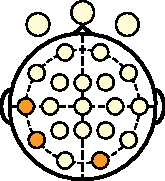
\includegraphics[width=0.17\textwidth]{./img_art_dfa/prop_MJH_30.pdf} &
%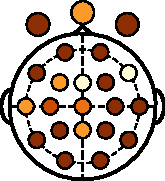
\includegraphics[width=0.17\textwidth]{./img_art_dfa/prop_JAE_30.pdf} &
%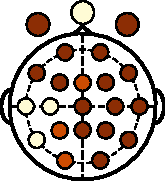
\includegraphics[width=0.17\textwidth]{./img_art_dfa/prop_MGG_30.pdf} &
%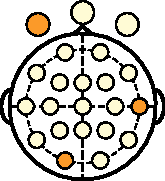
\includegraphics[width=0.17\textwidth]{./img_art_dfa/prop_EMT_30.pdf} \\
%\end{tabular} \\
%\midrule
%\begin{tabular}{ccccc}
%CLO & RLO JGZ & AEFP & PCM \\
%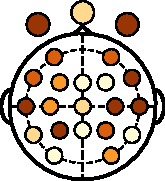
\includegraphics[width=0.17\textwidth]{./img_art_dfa/cabeza_new_VCR_30.pdf} &
%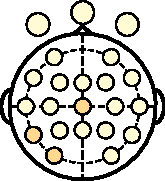
\includegraphics[width=0.17\textwidth]{./img_art_dfa/cabeza_new_MJH_30.pdf} &
%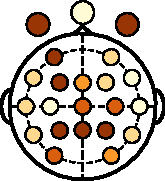
\includegraphics[width=0.17\textwidth]{./img_art_dfa/cabeza_new_JAE_30.pdf} &
%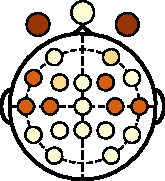
\includegraphics[width=0.17\textwidth]{./img_art_dfa/cabeza_new_GHA_30.pdf} &
%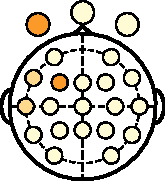
\includegraphics[width=0.17\textwidth]{./img_art_dfa/cabeza_new_MFGR_30.pdf} \\
%\end{tabular}
% \\
%
\includegraphics[scale=.7]{./img_art_dfa/escala.pdf} \\
%\end{tabular}
%\caption{Derivaciones para las cuales la proporción de épocas clasificadas como estacionarias fue significativamente diferente en MOR y NMOR.
%%
%Para esta figura se usaron épocas de 30 segundos de duración.
%%
%La posición de los círculos representan a las derivaciones, en correspondencia con la figura \ref{img:estampa}.}
%\label{cabeza_new}
%\end{figure}

%\begin{figure}
%\centering
%\begin{tabular}{ccccc}
%VCR & MJH & JAE & GHA & MFGR \\
%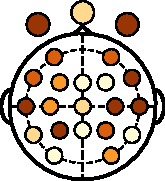
\includegraphics[width=0.17\textwidth]{./img_art_dfa/cabeza_new_VCR_30.pdf} &
%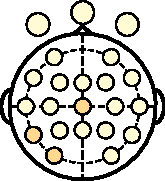
\includegraphics[width=0.17\textwidth]{./img_art_dfa/cabeza_new_MJH_30.pdf} &
%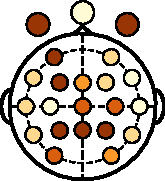
\includegraphics[width=0.17\textwidth]{./img_art_dfa/cabeza_new_JAE_30.pdf} &
%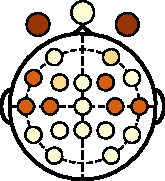
\includegraphics[width=0.17\textwidth]{./img_art_dfa/cabeza_new_GHA_30.pdf} &
%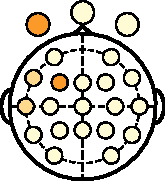
\includegraphics[width=0.17\textwidth]{./img_art_dfa/cabeza_new_MFGR_30.pdf} \\
%\midrule
%CLO & RLO & RRU & JGZ & AEFP \\
%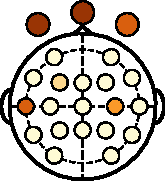
\includegraphics[width=0.17\textwidth]{./img_art_dfa/cabeza_new_CLO_30.pdf} &
%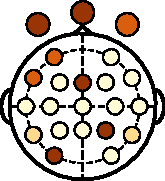
\includegraphics[width=0.17\textwidth]{./img_art_dfa/cabeza_new_RLO_30.pdf} &
%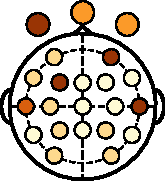
\includegraphics[width=0.17\textwidth]{./img_art_dfa/cabeza_new_RRU_30.pdf} &
%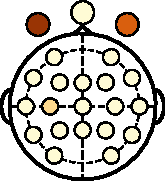
\includegraphics[width=0.17\textwidth]{./img_art_dfa/cabeza_new_JGZ_30.pdf} &
%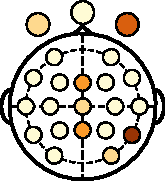
\includegraphics[width=0.17\textwidth]{./img_art_dfa/cabeza_new_AEFP_30.pdf} \\
%\end{tabular} \\
%
\includegraphics[scale=.7]{./img_art_dfa/escala.pdf} \\
%\caption{Derivaciones para las cuales la proporción de épocas clasificadas como estacionarias fue significativamente diferente en MOR y NMOR.
%%
%Para esta figura se usaron épocas de 30 segundos de duración.
%%
%La posición de los círculos representan a las derivaciones, en correspondencia con la figura \ref{img:estampa}.}
%\label{cabeza_new}
%\end{figure}

Con base a la hipótesis sobre estacionariedad local, discutida en la sección \ref{sec:est_local}, se procedió a repetir la clasificación de estacionariedad pero usando ventanas de diferentes tamaños.
%
Por fines de comparabilidad y por motivos técnicos, los tamaños de ventana se eligieron de la forma $30 \times 2^{n}$ segundos.
%
El tamaño de ventana más pequeño considerado fue de $\nicefrac{30}{32}$ segundos para poder correr la prueba de PSR de forma confiable, mientras que el tamaño más grande fue de $240$ segundos tomando en cuenta que bloques más grandes son demasiado heterogéneos para considerarse como unidades de estudio fiables.

%usando la frecuencia de muestreo de 512 Hz, la ventana más pequeña representa ventanas 480 puntos y una frecuancia de Nyquist de 280 \Hz ??, lo cual se consideró como un mínimo para hacer estadísticas.

En la figura \ref{cabeza_repoio} se muestra únicamente las proporciones estimadas de épocas estacionarias para MOR y NMOR, para un participante; los resultados de este análisis para todos los participantes puede encontrarse en el apéndice \ref{apendiceA}.
%
Usando épocas de mayor duración, se encuentra que una proporción menor de estas son clasificadas como estacionarias; sin embargo, usando épocas de menor duración no se garantiza el efecto contrario.
%
%Lo anterior puede explicarse bien porque las señales consideradas presentan una estructura cambiante a escalas muy pequeñas, o bien como artefacto de un tamaño de muestra pequeño en la prueba de PSR.
% 
%Dicho fenómeno no será explorado en el presente trabajo, ya que se requieren registros con una mayor frecuencia de muestreo para verificar la segunda hipótesis.
%
Dicho fenómeno será discutido posteriormente.

\begin{figure}
\centering
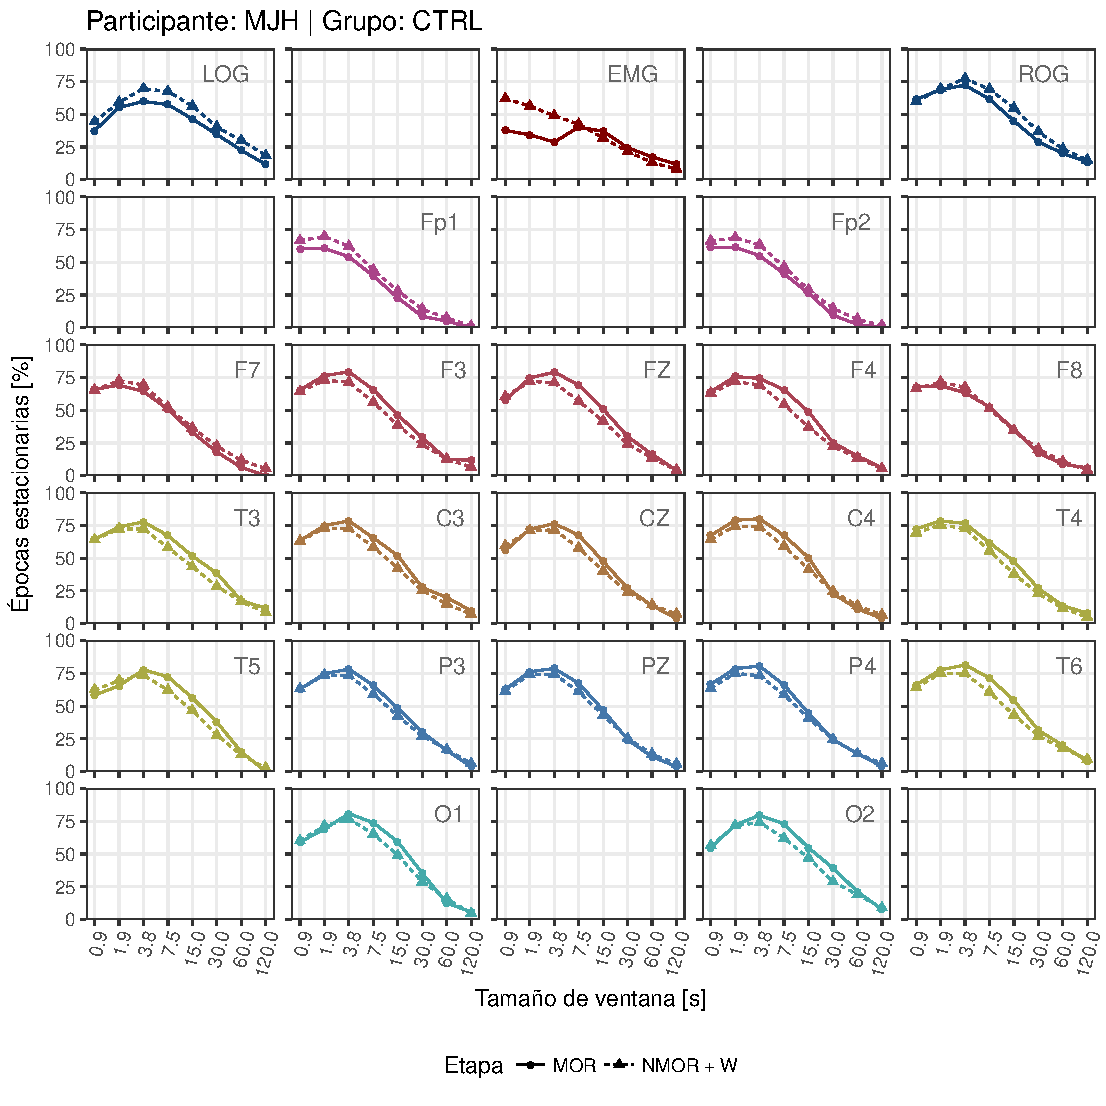
\includegraphics[width=\linewidth]{./scripts_graf_res/MJNNVIGILOS_cabeza_epocas_v2.pdf}
\caption{Cambio en el porcentaje de épocas estacionarias, respecto al tamaño de ventana considerado, en cada una de las derivaciones consideradas. La posición y color de cada gráfico se corresponden a aquellos de la figura \ref{img:estampa}. Sea abrevia W=Vigilia, recordando que la cantidad tiempo de los registros clasificada como vigilia es negligible.}
\label{cabeza_repoio}
\end{figure}

Intuitivamente, no se pudo identificar una conexión clara entre el PDCL y las características de las épocas como unidades autónomas.
%
Es debido a ello que se consideran otros dos niveles de organización sobre los registros: los registros como un conjunto de épocas distribuidas en el tiempo con \textit{cierta estructura}, y al individuo como unidad en la variabilidad de dichas estructuras.

%%%%%%%%%%%%%%%%%%%%%%%%%%%%%%%%%%%%%%%%%%%%%%%%%%%%%%%%%%%%%%%%%%%%%%%%%%%%%%%%%%%%%%%%%%%%%%%%%%%
%%%%%%%%%%%%%%%%%%%%%%%%%%%%%%%%%%%%%%%%%%%%%%%%%%%%%%%%%%%%%%%%%%%%%%%%%%%%%%%%%%%%%%%%%%%%%%%%%%%

\section{Análisis a nivel de registro}
\label{sec:analisis_registro}

Como se mencionó en la sección \ref{sec:pdcl_sueno}, se ha reportado cambios en la estructura del sueño en adultos mayores con deterioro cognitivo, respecto a adultos mayores saludables.
%
El objetivo de esta subsección es intentar detectar estos \textit{cambios de estructura} usando los métodos descritos y bajo las condiciones descritas.

Con el fin de explorar cómo se relacionan las épocas estacionarias con la \textit{estructura del sueño}, se procedió a \textit{graficar} la estacionariedad.
%
Para efectuar lo anterior se consideró una cuadrícula, con una fila por cada derivación y una columna por cada época analizada (se registró el mismo número de épocas para cada derivación); sobre la cuadrícula el espacio correspondiente a cada época fue coloreado a según la clasificación de la época como estacionaria.
%
Se procedió similarmente para ilustrar la clasificación según etapa de sueño.
%
En la figura \ref{img:patrones} se ejemplifica este tipo de gráficos, además de otros detalles a mencionarse.

\begin{figure}
\centering
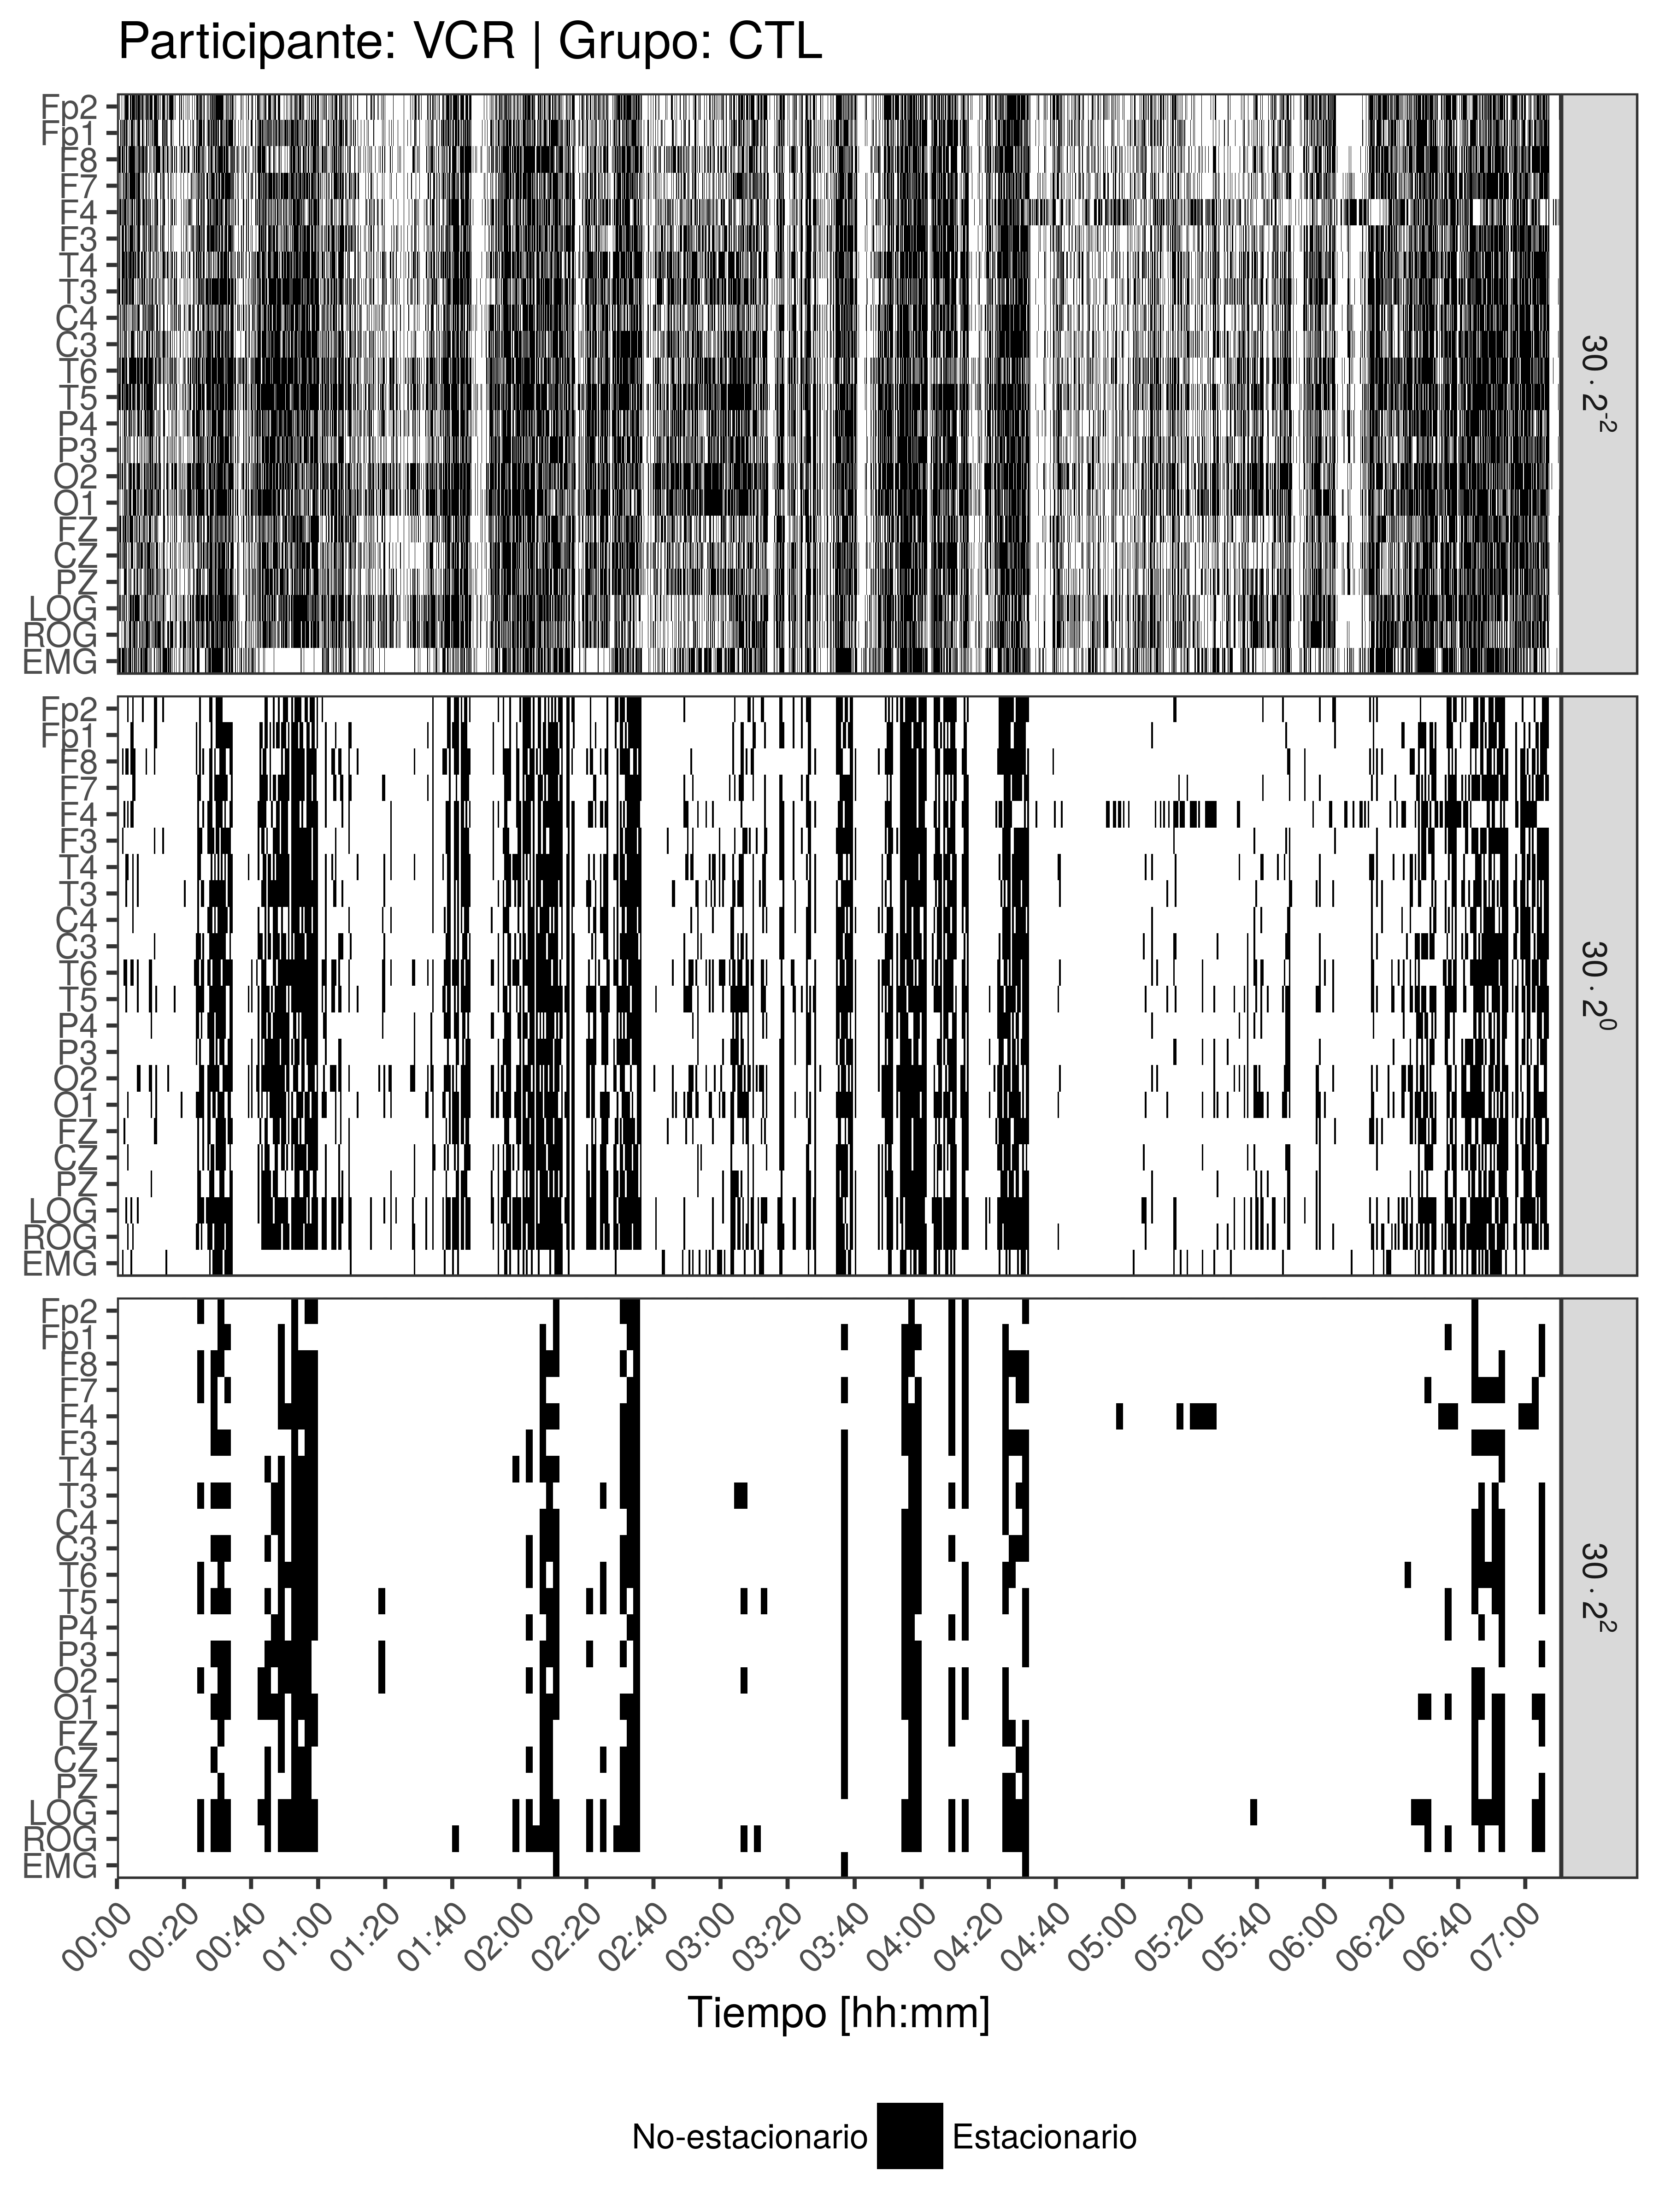
\includegraphics[width=.8\linewidth]
{./img_art_dfa/VCNNS1_comp_est_.png}
\caption[Distribución en el tiempo de las ventanas clasificadas como estacionarias, considerando diferentes tamaños de ventana]{Distribución en el tiempo de las ventanas clasificadas como estacionarias, considerando diferentes tamaños de ventana. 
Cada ventana fue representada en una cuadrícula según su derivación (margen izquierdo) y momento (margen inferior) de procedencia; posteriormente fue \textit{coloreada} según su clasificación como estacionaria.
Dado que la clasificación de estacionariedad se repitió usando diversos tamaños de ventana, éstos se indican en el margen derecho.
En la parte inferior se representan las mismas épocas en su clasificación según etapa de sueño.
Adicionalmente, en la parte superior se indican los \textit{patrones emergentes} de estacionariedad; para más detalles al respecto, ver el texto.}
\label{img:patrones}
\end{figure}

Los gráficos obtenidos mediante este procedimiento mostraron algunas regularidades que merecen especial atención: \textit{bloques emergentes} de épocas que comparten clasificación como estacionarias (o como no--estacionarias).
%
Estos bloques identificados visualmente se extienden entre diversas derivaciones; puede verse un ejemplo de ello en la figura \ref{img:patrones}.
%
Debido a la forma en que se efectuó la clasificación de estacionariedad (usando la prueba de PSR) puede garantizarse que estos patrones emergentes no son producidos por la clasificación per se.
%
Se hipotetiza que estos \textit{patrones de estacionariedad}
corresponden a las diferentes etapas de sueño.
%
Posteriormente se discutirá con más detalle al respecto.

El procedimiento de graficación se repitió para las clasificaciones de estacionariedad obtenidas usando diferentes tamaños de ventana, con el fin de verificar si la presencia de los bloques podría atribuirse al tamaño de ventana usado.
%
Se encontró que los patrones aparecen con mayor o menor \textit{nitidez} en los gráficos obtenidos usando diferentes tamaños de ventana, tal como se ilustra en la figura \ref{img:patrones}.

%Como análisis exploratorio se graficaron en el tiempo las épocas, en todos los canales, como se 
%muestra en la figura \ref{patroncito}. Este tipo de gráficos \textit{revelan} cierto tipo de 
%\textit{bloques} de épocas estacionarias o no-estacionarias. Heurísticamente se puede afirmar que 
%éstos patrones son independientes de la prueba de PSR, y anteriormente se reportó que estos patrones
%suelen coincidir con la aparición de sueño MOR. Más adelante se ofrece una discusión al 
%respecto.

%\begin{figure}
%\centering
%\includegraphics[width=.9\textwidth]
%{./img_art_dfa/zoom_noVCR_v2.png} \\
%\includegraphics[width=.9\textwidth]
%{./img_art_dfa/zoom_siVCR_v2.png}
%\caption[Ubicación de épocas estacionarias en el tiempo y patrones emergentes]
%{Ubicación de épocas estacionarias en el tiempo y patrones emergentes. \textbf{Arriba:} 
%Ubicación de épocas estacionarias en el tiempo.
%\textbf{Abajo:} Patrón de bloques relacionado con el sueño MOR}
%\label{patroncito}
%\end{figure}

%Usando la clasificación de épocas estacionarias, obtenida para diferentes tamaños de ventana, se 
%construyeron más gráficos sobre la ubicación de épocas estacionarias en el tiempo. Estos nuevos
%gráficos, como el de la figura \ref{comp_VCR}, refuerzan heurísticamente la hipótesis de que los 
%patrones son significativos fisiológicamente. 

%Entonces, se propone que los registros de PSG se comportan como procesos localmente estacionarios; 
%más aún, se propone que esta característica cambia cualitativamente en adultos mayores con PDC,
%para los cuales el \textit{nivel de homogeneidad} del PSG es muy similar durante MOR y NMOR.

%\begin{figure}
%\centering
%\includegraphics[width=\linewidth]
%{./img_art_dfa/VCNNS1_comp_est_.png}
%\caption{Distribución en el tiempo de ventanas estacionarias, usando diferentes tamaños
%de ventana.}
%\label{comp_VCR}
%\end{figure}

Dentro del contexto del PDCL en adultos mayores, estos patrones de estacionariedad no serán definidos formalmente ni estudiados detalladamente; se presentan como un hallazgo incidental y como verificación empírica de las capacidades de la técnica descrita para distinguir características que varían en el tiempo.
%
Esta decisión fue tomada considerando la naturaleza fuertemente cualitativa de dichos patrones.
%, la cual implicaría una serie de precauciones previas y posteriores al uso de pruebas estadísticas.

% apoyo a la afirmación de que la técnica empleada para determinar la estacionariedad puede distinguir 

%\footnote{Nótese que este concepto no ser define formalmente durante el presente trabajo.}

%%%%%%%%%%%%%%%%%%%%%%%%%%%%%%%%%%%%%%%%%%%%%%%%%%%%%%%%%%%%%%%%%%%%%%%%%%%%%%%%%%%%%%%%%%%%%%%%%%%

\section{Análisis a nivel de grupo}

Se repitió la comparación a un nivel grupal, usando la prueba $U$ de  Mann-Whitney.
Se encontraron diferencias significativas para el grupo CTL en los canales P3, P4, PZ, 
ROG y EMG; en el grupo PDC se observaron tales diferencias sólo en P4.
%
Las proporciones muestran tendencias que, quizá, resultaron no ser significativas
por el tamaño pequeño de la muestra: los canales P3 y PZ podrían ser diferentes también para
individuos del grupo PDC, y el canal LOG podría ser diferente durante sueño MOR y NMOR.
%
Así mismo se hipotetiza que para el grupo CTL, en todos los canales, el sueño MOR
es presenta menor cantidad de épocas estacionarias.

Se concluye que
no se puede establecer diferencias entre las medias grupales para esta cantidad (proporción de
épocas estacionarias, medidas en el sentido de PSR), debido a la gran variabilidad entre sujetos.


\begin{figure}
\centering
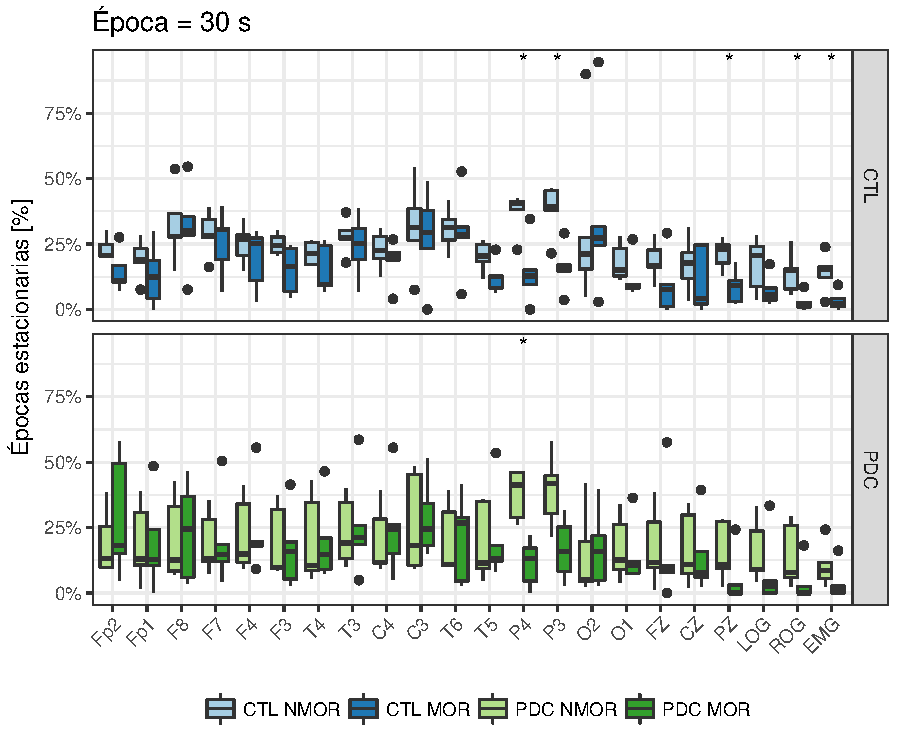
\includegraphics[width=\linewidth]
{./img_art_dfa/Comparacion_gpos_CTL_PDC_v3.pdf}
\caption{Proporciones de épocas estacionarias, durante sueño MOR y NMOR.}
\label{comparacion_verde}
\end{figure}

\begin{figure}
\centering
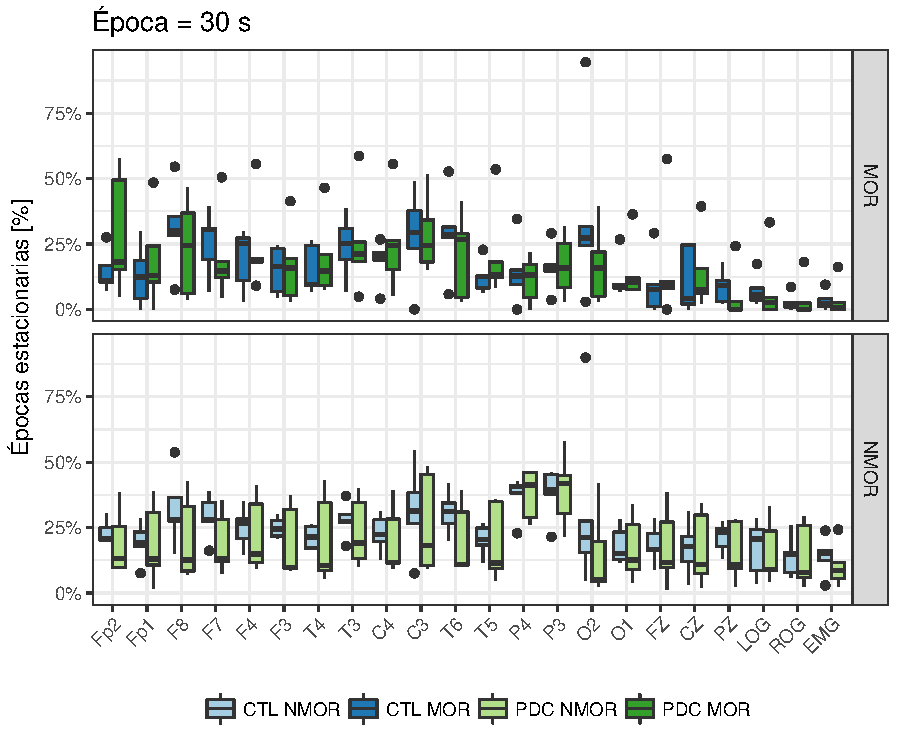
\includegraphics[width=\linewidth]
{./img_art_dfa/Comparacion_gpos_MOR_NMOR_v3.pdf}
\caption{Proporciones de épocas estacionarias, grupos CTL y PDC.}
\label{comparacion_graf}
\end{figure}

%%%%%%%%%%%%%%%%%%%%%%%%%%%%%%%%%%%%%%%%%%%%%%%%%%%%%%%%%%%%%%%%%%%%%%%%%%%%%%%%%%%%%%%%%%%%%%%%%%%
%%%%%%%%%%%%%%%%%%%%%%%%%%%%%%%%%%%%%%%%%%%%%%%%%%%%%%%%%%%%%%%%%%%%%%%%%%%%%%%%%%%%%%%%%%%%%%%%%%%
%%%%%%%%%%%%%%%%%%%%%%%%%%%%%%%%%%%%%%%%%%%%%%%%%%%%%%%%%%%%%%%%%%%%%%%%%%%%%%%%%%%%%%%%%%%%%%%%%%%